\documentclass[11pt,a4paper]{article}

% ---------- Packages ----------
\usepackage[margin=1in]{geometry}
\usepackage{times}
\usepackage{titlesec}
\usepackage{enumitem}
\usepackage{booktabs}
\usepackage{array}
\usepackage{longtable}
\usepackage{multirow}
\usepackage{amssymb}
\usepackage{xcolor}
\usepackage{colortbl}
\usepackage{tikz}
\usetikzlibrary{arrows.meta,positioning,fit,backgrounds}
\usepackage{hyperref}
\usepackage{fancyhdr}
\usepackage{graphicx}
\usepackage{setspace}
\usepackage{caption}
\usepackage{capt-of}
\usepackage{pifont}
\usepackage{needspace}

\hypersetup{
    colorlinks=true,
    linkcolor=blue!50!black,
    citecolor=blue!50!black,
    urlcolor=blue!50!black,
    pdftitle={VidCraft FYP Proposal},
}

\definecolor{headerblue}{RGB}{68,114,196}
\definecolor{lightblue}{RGB}{221,235,247}

\titleformat{\section}{\large\bfseries}{\thesection}{0.5em}{}
\titleformat{\subsection}{\normalsize\bfseries}{\thesubsection}{0.5em}{}
\titleformat{\subsubsection}{\normalsize\bfseries\itshape}{\thesubsubsection}{0.5em}{}

\pagestyle{fancy}
\fancyhf{}
\rhead{VidCraft FYP Proposal}
\lhead{Group 7}
\cfoot{\thepage}

\setstretch{1.08}

\newcommand{\tblhead}[1]{\cellcolor{headerblue}\textcolor{white}{\textbf{#1}}}

\begin{document}

% ==========================================================
% TITLE PAGE
% ==========================================================
\begin{titlepage}
\centering
\vspace*{1.5cm}

{\Huge\bfseries VidCraft\par}
\vspace{0.4cm}
{\Large A Multi-Agent, Retrieval-Augmented Pipeline for\\ Prompt-Driven Video Generation\par}

\vspace{1.2cm}
{\large Final Year Project Proposal\par}
{\large Session 2023\par}

\vspace{1.2cm}
{\large\bfseries Submitted by\par}
\vspace{0.4cm}
{\large
Maida Ibrar (2023-CS-505)\\
Hammad (2023-CS-567)\\
Muhammad Majid (2023-CS-580)\\
Tahir Zaka (2023-CS-596)\par
}

\vspace{1.2cm}
{\large\bfseries Supervisor\par}
Ms. Rabia Sana\par
\vspace{0.5cm}
{\large\bfseries Co-Supervisor\par}
Dr. Yaeen-ul-Haq\par

\vspace{1.5cm}
% Replace the placeholder box below with your department logo, e.g.:
% \includegraphics[width=3cm]{uet_logo.png}
\fbox{\parbox{3cm}{\centering\vspace{1.2cm}UET\\Logo\vspace{1.2cm}}}

\vspace{1.5cm}
{\large
Department of Computer Science \& Engineering\\
University of Engineering and Technology, Lahore\\
(Narowal Campus)\par
}
\vspace{0.4cm}
{\large\bfseries 2023--2027\par}

\end{titlepage}

% ==========================================================
% PROJECT REGISTRATION
% ==========================================================
\section*{Project Registration}

\noindent Project ID (for office use): \underline{\hspace{4cm}} \hfill Type of project: Industrial

\vspace{0.3cm}
\noindent Nature of project: $\square$ Development \quad $\square$ Research \quad $\blacksquare$ R\&D

\noindent Area of Specialisation: AI, Generative Models, NLP, Multi-Agent Systems

\vspace{0.4cm}
\noindent\textbf{Project Group Members}

\begin{center}
\begin{tabular}{|c|l|l|c|l|l|c|}
\hline
\rowcolor{headerblue}
\textcolor{white}{\textbf{Sr.\#}} & \textcolor{white}{\textbf{Reg.\#}} & \textcolor{white}{\textbf{Student Name}} & \textcolor{white}{\textbf{CGPA}} & \textcolor{white}{\textbf{Email ID}} & \textcolor{white}{\textbf{Phone \#}} & \textcolor{white}{\textbf{Sign.}} \\
\hline
(i) Leader & 2023-CS-580 & Muhammad Majid & 3.87 & 2023cs580@student.uet.edu.pk & 03079472072 & \\
\hline
(ii) & 2023-CS-596 & Tahir Zaka & 3.43 & 2023cs596@student.uet.edu.pk & 03054536018 & \\
\hline
(iii) & 2023-CS-567 & Hammad & 3.64 & 2023cs567@student.uet.edu.pk & 03430789110 & \\
\hline
(iv) & 2023-CS-505 & Maida Ibrar & 3.36 & 2023cs505@student.uet.edu.pk & 03186186178 & \\
\hline
\end{tabular}
\end{center}

\vspace{0.4cm}
\noindent\textit{Declaration: FYP group members have cleared all prerequisite courses for FYP-I as per their degree requirements.}

\clearpage

% ==========================================================
% PLAGIARISM CERTIFICATE
% ==========================================================
\section*{Plagiarism Certificate}

\noindent This is to certify that, I am \underline{\hspace{3cm}} S/D/o \underline{\hspace{3cm}}, group leader of FYP under registration no. \underline{\hspace{2.5cm}} at the Computer Science Department, University of Engineering and Technology Lahore, Narowal Campus. I declare that my FYP proposal has been checked by my supervisor and the similarity index is \underline{\hspace{1.5cm}}\%, which is less than 20\%, the acceptable limit set by HEC. The similarity report is attached herewith as Appendix A.

\vspace{1cm}
\noindent Date: \underline{\hspace{3cm}} \hfill Name of Group Leader: \underline{\hspace{3cm}} \hfill Signature: \underline{\hspace{2cm}}

\vspace{1.5cm}
\noindent
\begin{minipage}{0.48\textwidth}
Name of Supervisor: \underline{\hspace{3cm}}\\[0.3cm]
Designation: \underline{\hspace{3cm}}\\[0.3cm]
Signature: \underline{\hspace{3cm}}
\end{minipage}
\hfill
\begin{minipage}{0.48\textwidth}
Co-Supervisor (if any): \underline{\hspace{3cm}}\\[0.3cm]
Designation: \underline{\hspace{3cm}}\\[0.3cm]
Signature: \underline{\hspace{3cm}}
\end{minipage}

\clearpage

\tableofcontents
\clearpage

\section*{List of Abbreviations}
\begin{center}
\begin{tabular}{|l|l|}
\hline
\tblhead{Abbreviation} & \tblhead{Meaning} \\
\hline
AI & Artificial Intelligence \\
API & Application Programming Interface \\
CLIP & Contrastive Language--Image Pre-training \\
FYP & Final Year Project \\
FFmpeg & Fast Forward Moving Picture Experts Group (media processing tool) \\
JSON & JavaScript Object Notation \\
LLM & Large Language Model \\
NER & Named Entity Recognition \\
NLP & Natural Language Processing \\
POS & Part of Speech \\
RAG & Retrieval-Augmented Generation \\
REST & Representational State Transfer \\
TTS & Text to Speech \\
UI/UX & User Interface / User Experience \\
\hline
\end{tabular}
\end{center}

\needspace{0.5\textheight}

% ==========================================================
% MAIN CONTENT
% ==========================================================

\section{Project Abstract}

VidCraft is an end-to-end AI-assisted video generation pipeline that turns a single natural-language idea into a coherent, multi-shot video. Rather than treating prompt improvement as a single text-rewriting step, VidCraft coordinates a small team of cooperating LLM agents, orchestrated with LangGraph, that decompose a user's idea into a short storyboard, assign per-shot cinematic parameters, and route each shot to the appropriate generation backend.

The system retains a dual-generation strategy for cost control. A Remotion-based programmatic rendering pathway produces animated videos directly from code at no per-generation cost and gives the system a pathway with fully deterministic scene and character consistency, since the same parameters are reused directly in the rendering code across shots. A tiered external video-API pathway is used when photorealistic output is required, prioritising free-tier and trial-credit providers before paid options; consistency of appearance across independently generated clips on this pathway is treated honestly as a best-effort property rather than a guarantee, consistent with the current state of published text-to-video research.

Two further additions distinguish this iteration of the project from a purely sequential prompt-to-API pipeline. First, a retrieval-augmented style grounding step lets the Cinematographer agent draw on a curated, embedded knowledge base of cinematography conventions (shot types, lighting, genre vocabulary) rather than relying only on the language model's parametric knowledge. Second, a bounded critic-and-retry loop evaluates generated output against the intended shot description and can trigger a limited number of automatic re-generations when the output does not match, rather than accepting the first result unconditionally. A conversational clarification agent additionally resolves ambiguous prompts through a short, targeted question-and-answer exchange before generation begins, rather than silently guessing missing details.

The React-based frontend provides this conversational prompt-clarification flow, a style configurator, a storyboard/shot timeline, and real-time generation progress over WebSocket. The project is implemented by a four-member team across ten structured development phases from May 2026 to April 2027, and includes a comparative evaluation study contrasting single-shot prompt enhancement against the multi-agent pipeline on a fixed prompt set, together with a documented testing strategy and an explicit risk and ethics analysis.

\needspace{0.5\textheight}
\section{Introduction}

The rapid advancement of generative artificial intelligence has made it possible to produce video content directly from textual descriptions. Systems such as Sora, Veo and Kling have shown that a short, photorealistic video clip can be produced from a single sentence. However, three practical problems limit how useful this capability is for an ordinary user, and VidCraft is structured around addressing each of them directly.

\subsection*{Problem 1: Prompt quality is inconsistent and hard to get right}
The quality of AI-generated video is highly sensitive to the precision and richness of the input prompt. A prompt such as \textit{``a dog running''} typically produces a generic, low-detail clip, while a prompt such as \textit{``a golden retriever sprinting across a sunlit meadow, low-angle tracking shot, warm afternoon lighting, joyful energetic mood''} produces a substantially more compelling result from the same underlying model. Most users do not know which dimensions of a prompt (subject, action, setting, visual detail, mood) matter, or how to phrase them in the vocabulary a generation model responds well to.

\subsection*{Problem 2: A single generation call cannot express a multi-shot idea}
Even a well-written prompt describes, at best, one shot. Ideas that are naturally multi-scene -- for example, \textit{``a short story about an astronaut who loses radio contact on Mars and has to repair the antenna before nightfall''} -- cannot be expressed as a single text-to-video call. Producing this kind of output requires decomposing the idea into a small number of distinct shots, deciding what happens in each one, and keeping the character and setting description consistent across them. None of the commercial single-call APIs perform this decomposition automatically.

\subsection*{Problem 3: Iterative experimentation with commercial APIs is expensive}
Commercial text-to-video APIs charge per second of generated video, which makes the kind of iterative trial-and-error that produces a good result financially impractical for students, educators and independent creators experimenting with prompts, styles or storyboards.

\subsection*{How VidCraft addresses these problems}
On the first problem, a spaCy-based natural language analysis pipeline scores prompts across five dimensions (subject clarity, action specificity, environment detail, visual richness and temporal coherence), and a conversational clarification agent asks targeted follow-up questions when key information is missing, rather than guessing. On the second problem, a small set of cooperating LLM agents, coordinated with LangGraph, break a suitable prompt into a short storyboard and assign cinematic parameters to each shot, drawing on a retrieval-augmented knowledge base of cinematography conventions rather than the language model's unaided judgement, and a shared world-state object keeps character and setting descriptions consistent across shots. On the third problem, VidCraft retains a programmatic generation pathway using Remotion, allowing animated videos to be rendered entirely from code at near-zero marginal cost, alongside a tiered external API pathway reserved for photorealistic output.

\subsection*{Target Users}
\begin{itemize}[leftmargin=*]
\item \textbf{Students and self-learners} who want to practise storytelling and visual communication without owning production equipment.
\item \textbf{Educators} who want to produce short explanatory or narrative videos for classroom use on a limited or no budget.
\item \textbf{Small content creators and freelancers} who need short promotional or social-media video content without hiring a production team.
\item \textbf{Researchers} interested in prompt engineering, agentic pipelines or retrieval-augmented generation as a testbed for further experimentation.
\end{itemize}

\subsection*{A Note on Scope of Claims}
Throughout this proposal, capabilities that can be delivered with a firm guarantee (for example, deterministic consistency on the Remotion pathway) are distinguished explicitly from capabilities that are best-effort or exploratory (for example, appearance consistency across independently generated photorealistic clips, or the outcome of the comparative evaluation study). This distinction is maintained deliberately so that the project's success criteria remain achievable, verifiable, and honestly reported at the final demonstration.

\needspace{0.5\textheight}
\section{Success Criterion}

Given the exploratory nature of the multi-agent and retrieval-augmented components, success is defined at three levels: a \textbf{Minimum Viable} level that must be achieved for the project to be considered complete, a \textbf{Target} level expected under normal execution of the plan, and a \textbf{Stretch} level that exceeds the criterion if time and budget permit.

\subsection*{Minimum Viable Outcomes}
\begin{itemize}[leftmargin=*]
\item The spaCy-based prompt analyzer produces a structured five-dimension quality score and improvement suggestions for arbitrary input prompts, validated against a curated test set of 50 prompts.
\item The LangGraph multi-agent orchestrator successfully decomposes at least one complex input prompt into a multi-shot storyboard (3--5 shots) and renders every shot end-to-end through the Remotion pathway, with character and style parameters shared consistently across all shots.
\item The React frontend, including the conversational clarification flow, style configurator, real-time progress tracker and storyboard/version timeline, is fully functional and mobile-responsive.
\item The complete end-to-end pipeline, from frontend prompt submission to video delivery via WebSocket, completes at least one successful run demonstrated live during the final demonstration.
\end{itemize}

\subsection*{Target Outcomes}
\begin{itemize}[leftmargin=*]
\item The retrieval-augmented style grounding module returns relevant cinematography reference content for prompts in a held-out test set, with relevance verified manually on a sample of at least 30 queries.
\item The critic-and-retry feedback loop is implemented and demonstrably triggers at least one automatic re-generation cycle based on structured feedback, bounded to a configurable maximum number of retries.
\item The external API integration layer successfully generates at least one real video through a connected provider, with cross-shot continuity handled on a best-effort basis (shared descriptive parameters and, where supported by the provider, a shared reference image) rather than guaranteed pixel-level consistency.
\item A comparative evaluation is conducted between single-shot prompt enhancement and the full multi-agent pipeline on a fixed prompt set, with quantitative and qualitative results documented in the final report. The study itself, rigorously conducted and reported, constitutes the success criterion; a specific directional result is not presupposed.
\item A documented testing strategy (unit, integration and end-to-end) is executed and reported with pass/fail results for each pipeline component.
\end{itemize}

\subsection*{Stretch Outcomes}
\begin{itemize}[leftmargin=*]
\item Tool-augmented reference-image retrieval (from a stock-image API) feeds into shot generation prompts to further ground style decisions.
\item Synchronized audio narration is generated by a text-to-speech service and merged into the rendered video.
\item The critic-and-retry loop is extended to operate on the external API pathway within a strict, budget-capped retry limit.
\end{itemize}

\needspace{0.5\textheight}
\section{Related Work}

\subsection{Text-to-Video Generation Systems}
Text-to-video models such as Sora (OpenAI, 2024), Veo (Google DeepMind, 2024) and Kling (Kuaishou, 2024) have demonstrated the feasibility of generating short photorealistic video clips from natural language descriptions \cite{sora,veo,controllable_survey}. These systems assume the user can supply a high-quality prompt, generate a single clip per call, and charge significant per-second fees, which together make iterative experimentation and multi-shot narrative construction costly. Cross-clip consistency of character appearance across independently generated calls remains, by the survey literature's own account, a largely open problem even at the frontier level \cite{controllable_survey}.

\subsection{Prompt Engineering and Enhancement}
Prompt engineering for generative models has been studied extensively; structured, dimension-specific prompts have been shown to outperform free-form descriptions in generation quality \cite{devil_in_prompts}. Commercial prompt marketplaces exist, but they rely on manually authored, static prompt templates rather than an automated, linguistically grounded scoring and enhancement process tailored to video generation.

\subsection{Iterative and Self-Refining Generation}
Iterative, feedback-driven refinement has been explored directly in the video domain: PhyT2V demonstrates LLM-guided iterative self-refinement for physics-grounded text-to-video generation \cite{phyt2v}, and more broadly, Self-Refine shows that language models can improve their own output through iterative self-critique without additional training \cite{selfrefine}. VidCraft's critic-and-retry loop applies this established iterative-refinement pattern to shot-level video generation, a comparatively underexplored setting, rather than presenting it as a wholly novel technique.

\subsection{Multi-Agent LLM Systems}
Coordinating multiple language-model agents, each assigned a specialised role, to complete a larger task has been studied in work such as generative agent simulations \cite{genagents}, and is increasingly supported by orchestration frameworks including LangGraph \cite{langgraph}, which provides explicit state graphs, conditional branching and cycles for exactly this kind of coordination. VidCraft applies this pattern to video pre-production: a Screenwriter agent, a Cinematographer agent and a Producer/Router agent divide the work of decomposing a prompt into a storyboard and assigning per-shot parameters.

\subsection{Retrieval-Augmented Generation}
Retrieval-augmented generation, which grounds a language model's output in retrieved external content rather than relying solely on parametric knowledge, was formalised by Lewis et al. \cite{rag}. It is now a standard technique for reducing hallucination and improving factual or stylistic grounding in knowledge-intensive tasks. VidCraft applies this pattern to cinematography style grounding: the Cinematographer agent retrieves relevant shot-type, lighting and genre reference material before assigning style parameters to a shot, rather than relying purely on the underlying language model's training data.

\subsection{Programmatic and Code-Driven Video Generation}
Programmatic video generation represents a complementary paradigm to model-based generation. Remotion \cite{remotion} introduced React-based declarative video production, enabling developers to produce animated videos using familiar web development skills, and the Manim library \cite{manim} similarly pioneered code-driven mathematical animation. Because a programmatic composition is defined entirely by its input parameters, reusing the same parameters across multiple renders yields exact, deterministic consistency -- a property that is straightforward to obtain here precisely because it is not attempted through a generative model at all.

Sentence embedding models such as Sentence-BERT \cite{sbert} have been applied broadly to document retrieval and semantic search; their use here for prompt version comparison and cinematic style retrieval is a direct application of an established technique to a new domain rather than a methodological contribution in itself. Likewise, the use of spaCy \cite{spacy} dependency parsing for prompt quality scoring applies standard NLP tooling to a video-specific scoring rubric. Evaluation of generated video against a source prompt is itself an active research area; CLIPScore \cite{clipscore} and the EvalCrafter benchmark \cite{evalcrafter} both propose reference-free, embedding-based measures of text-visual alignment, which inform the evaluation methodology adopted in Section~6.10.

\subsection{Comparative Positioning}

Table~\ref{tab:comparison} summarises how VidCraft's design choices relate to existing systems along the dimensions most relevant to this proposal. The comparison is intended to make explicit which capabilities are already well established elsewhere and which combination is specific to this project, rather than to claim outright novelty of any individual technique.

\begin{center}
\begin{tabular}{|p{3.3cm}|p{1.9cm}|p{1.9cm}|p{2.3cm}|p{2.3cm}|}
\hline
\tblhead{System} & \tblhead{Multi-shot decomposition} & \tblhead{RAG-grounded style} & \tblhead{Bounded feedback loop} & \tblhead{Guaranteed-consistency pathway} \\
\hline
Sora / Veo / Kling & \ding{55} & \ding{55} & \ding{55} & \ding{55} \\
\hline
Generic prompt-marketplace tools & \ding{55} & \ding{55} & \ding{55} & \ding{55} \\
\hline
Remotion / Manim (code-only) & Manual & \ding{55} & \ding{55} & \checkmark \\
\hline
PhyT2V (self-refinement) & \ding{55} & \ding{55} & \checkmark & \ding{55} \\
\hline
\textbf{VidCraft (proposed)} & \checkmark (agentic) & \checkmark & \checkmark (bounded) & \checkmark (Remotion pathway) \\
\hline
\end{tabular}
\captionof{table}{Comparative positioning of VidCraft against related systems. A \checkmark on the Remotion pathway only is intentional: consistency is not claimed on the external API pathway.}
\label{tab:comparison}
\end{center}

\needspace{0.5\textheight}
\section{Project Rationale}

Video is the dominant medium for online communication, education and creative expression, yet professional-quality video production remains difficult to access: traditional production requires specialist software and equipment, while AI generation APIs require prompt-engineering skill and significant financial expenditure. VidCraft is motivated by lowering both barriers through automated prompt and storyboard assistance and a cost-stratified generation strategy, while remaining explicit about which parts of the system offer strong guarantees and which are best-effort.

The project is additionally motivated by the practical constraints of an academic development team. By keeping the Remotion pathway as the primary demonstration vehicle for the multi-agent and continuity features, VidCraft ensures that the system remains functional and demonstrable throughout development even when external API budgets are limited, using programmatic rendering as a reliable, cost-free fallback. This design decision has both engineering merit (a stable, always-available demonstration path) and pedagogical merit (it forces the team to design the orchestration and continuity logic independently of any single third-party provider's availability or pricing).

\subsection{Aims and Objectives}

The primary aim of VidCraft is to build an end-to-end video generation pipeline that decomposes a single user idea into a coherent multi-shot output, remains usable by people without prompt-engineering expertise, and stays affordable through a tiered, largely free-tier generation strategy. The specific objectives are:

\begin{enumerate}[leftmargin=*]
\item Score user prompts across five linguistic dimensions and surface concrete, actionable improvement suggestions.
\item Resolve ambiguous prompts through a short conversational clarification exchange rather than silent guessing.
\item Decompose suitable prompts into a multi-shot storyboard using coordinated LLM agents, with per-shot cinematic parameters grounded in a retrieval-augmented style knowledge base.
\item Maintain a shared world-state across shots so that character and setting descriptions remain consistent, with consistency guaranteed on the programmatic pathway and pursued best-effort on the API pathway.
\item Provide both free (programmatic) and tiered paid video generation pathways, prioritising free-tier providers.
\item Implement a bounded, automated feedback loop that can trigger a limited number of re-generations when output does not match the intended shot description.
\item Provide a user-friendly interface for prompt authoring, clarification, storyboard review and generation progress tracking.
\item Conduct a comparative evaluation of single-shot versus multi-agent prompt enhancement on a fixed test set, and document a corresponding testing strategy for the pipeline as a whole.
\end{enumerate}

\subsection{Scope of the Project}

The scope of VidCraft is deliberately bounded to keep the project achievable within the allocated team size and timeline. Table~\ref{tab:scope} lists each deliverable together with the acceptance criterion used to judge whether it has been completed.

\begin{center}
\begin{longtable}{|p{6.3cm}|p{7.7cm}|}
\hline
\tblhead{Deliverable} & \tblhead{Acceptance Criterion} \\
\hline
\endfirsthead
\hline
\tblhead{Deliverable} & \tblhead{Acceptance Criterion} \\
\hline
\endhead
React-based frontend (prompt entry, clarification chat, style selection, storyboard review, progress tracking) & All listed views implemented, functional and verified on both desktop and mobile viewport sizes \\
\hline
Node.js/Express backend (API gateway, job scheduling, real-time updates) & REST endpoints documented and tested via Postman; WebSocket updates observed end-to-end in the frontend \\
\hline
Python FastAPI AI microservice (analyzer, orchestrator, RAG module, critic loop) & Each sub-module independently unit-tested; full request handled without error for at least one complex prompt \\
\hline
Remotion-based rendering engine & At least three distinct animated compositions rendered from a single storyboard without external API cost \\
\hline
Tiered external video/image API integration & At least one real video generated end-to-end through a connected free-tier provider \\
\hline
FFmpeg post-processing module (concatenation, thumbnails, subtitles, compression) & Multi-shot storyboard output concatenated into one continuous, web-optimised MP4 \\
\hline
Optional text-to-speech narration (stretch) & Narration audio generated and merged with rendered video for at least one demonstration case \\
\hline
MongoDB data layer (prompts, storyboards, embeddings) & Schema documented; data persisted and retrievable across a full pipeline run \\
\hline
Comparative evaluation study & Baseline and multi-agent conditions run on the same fixed prompt set; results documented in the final report \\
\hline
Testing report (unit, integration, end-to-end) & Test cases documented with pass/fail outcomes for each major pipeline component \\
\hline
Final live demonstration & Complete pipeline run, from prompt submission to delivered video, demonstrated live without pre-recording \\
\hline
\end{longtable}
\end{center}
\vspace{-0.3cm}
\begin{center}
\captionof{table}{Project deliverables and their acceptance criteria.}
\label{tab:scope}
\end{center}

To keep this scope achievable, the project deliberately excludes: multiple redundant text-to-speech providers (a single free-tier provider is used), an open-ended library of image-generation models (a small, tiered set is used), and any claim of guaranteed visual consistency on the external API pathway.

\subsection{Socio-Economic Benefit of the Project}

\begin{center}
\begin{longtable}{|p{4.3cm}|p{9.7cm}|}
\hline
\tblhead{Beneficiary} & \tblhead{Benefit} \\
\hline
\endfirsthead
\hline
\tblhead{Beneficiary} & \tblhead{Benefit} \\
\hline
\endhead
Students and self-learners & Learn prompt writing, storyboard planning and AI-assisted content production through interactive feedback, at no or minimal cost \\
\hline
Educators and training centres & Produce short explanatory or narrative videos for classroom use without specialist software or a production budget \\
\hline
Schools, universities, non-profits & Access structured, multi-shot AI video creation through the free Remotion pathway even with no generation budget at all \\
\hline
Small businesses and independent creators & Produce multi-shot promotional or educational videos without hiring a production team, choosing free or paid generation according to budget \\
\hline
Researchers and future FYP groups & A documented, extensible testbed for further experimentation with agentic pipelines, retrieval-augmented generation and prompt evaluation \\
\hline
Wider digital economy & Supports online businesses, digital marketing and freelancing by lowering the cost floor of producing short video content \\
\hline
\end{longtable}
\end{center}

\subsection{Budget of Project}

The estimated development and testing budget is structured as follows. Costs assume a mixed free-tier and paid usage pattern typical of iterative development and a final evaluation/demonstration phase.

\begin{center}
\begin{tabular}{|p{5cm}|p{3.2cm}|p{5.3cm}|}
\hline
\tblhead{Expense Category} & \tblhead{Estimated Cost} & \tblhead{Notes} \\
\hline
Remotion-based rendering & Rs.\ 0 & Runs locally, no per-video API cost \\
\hline
LLM inference (agent orchestration) & Rs.\ 0 -- 2,000 & Free-tier, low-latency inference used for the multi-agent orchestration layer \\
\hline
LLM inference (fallback / higher-complexity reasoning) & Rs.\ 3,000 -- 5,000 & Used selectively where a stronger model is needed \\
\hline
Vision-capable model calls (critic loop) & Rs.\ 1,000 -- 3,000 & Used only for bounded, capped retry evaluations \\
\hline
Image generation APIs & Rs.\ 2,000 -- 4,000 & Free-credit and trial-tier providers prioritised \\
\hline
External video generation APIs & Rs.\ 8,000 -- 12,000 & Free-tier providers prioritised; paid tier reserved for final testing and demonstration \\
\hline
Text-to-speech (audio narration) & Rs.\ 0 & Free-tier provider \\
\hline
Local compute (spaCy, sentence-transformers, vector index) & Rs.\ 0 & Runs on development machines \\
\hline
Contingency & Rs.\ 3,000 -- 5,000 & Unplanned testing or demonstration costs \\
\hline
\end{tabular}
\end{center}

\begin{center}
\textbf{Total Estimated Cost: PKR 17,000 -- 31,000}
\end{center}

Table~\ref{tab:phasecost} breaks the same estimate down by development phase, showing where in the timeline the majority of paid-API spending is expected to occur.

\begin{center}
\begin{tabular}{|p{6cm}|p{4cm}|p{3.3cm}|}
\hline
\tblhead{Development Phase} & \tblhead{Primary Cost Driver} & \tblhead{Approx.\ Share} \\
\hline
Phases 1--4 (setup, backend, frontend, Remotion) & Local compute only & 0\% \\
\hline
Phases 5--6 (orchestration, NLP core, RAG) & LLM inference (agent calls) & 25\% \\
\hline
Phase 7 (critic loop, external API integration) & Video/image API trial usage & 40\% \\
\hline
Phase 8 (integration and optimization) & Mixed LLM and API usage & 15\% \\
\hline
Phase 9 (evaluation study) & LLM and vision-model calls & 15\% \\
\hline
Phase 10 (report writing, demo prep) & Final demonstration API usage & 5\% \\
\hline
\end{tabular}
\captionof{table}{Estimated cost distribution across development phases.}
\label{tab:phasecost}
\end{center}

\needspace{0.5\textheight}
\section{Proposed Methodology and Architecture}

VidCraft adopts a layered architecture separating the React frontend, the Node.js backend and the Python AI microservice into independently deployable components communicating over HTTP and WebSocket. Figure~\ref{fig:architecture} shows the overall pipeline, and Figure~\ref{fig:sequence} shows the corresponding request sequence for a single end-to-end generation.

\subsection{Prompt Analysis Layer}

Raw user text is submitted to a FastAPI endpoint hosting a spaCy \texttt{en\_core\_web\_sm} analysis pipeline. The pipeline applies dependency parsing to detect subject presence, part-of-speech tagging to confirm action-verb coverage, named entity recognition to identify setting and location references, and a custom domain-specific antonym dictionary to detect visually contradictory word pairs (for example, ``bright'' and ``dim'' both present in the same description). The output is a structured JSON object containing an overall 0--100 quality score, a five-dimension breakdown, and natural-language improvement suggestions. An illustrative (abbreviated) output is shown below.

\begin{verbatim}
{
  "overall_score": 42,
  "dimensions": {
    "subject_clarity":    65,
    "action_specificity":  30,
    "environment_detail":  25,
    "visual_richness":     40,
    "temporal_coherence":  50
  },
  "flags": ["missing_setting", "vague_action"],
  "suggestions": [
    "Specify where the scene takes place (indoor/outdoor, time of day).",
    "Replace generic verb 'moves' with a more specific action."
  ]
}
\end{verbatim}

Prompts scoring below a configurable threshold (default: 60/100) are routed to the conversational clarification step described in Section~6.2, or directly to the multi-agent enhancement layer if the user opts to skip clarification.

\subsection{Conversational Clarification Agent}

When the analyzer flags missing or ambiguous information (for example, no setting, or a contradictory pair of descriptors), a lightweight clarification agent asks at most two targeted follow-up questions through the frontend chat interface -- for example, ``Should this be set indoors or outdoors?'' or ``Realistic or animated style?'' -- rather than silently guessing the missing detail. Responses are parsed into a structured \textit{brief} object using the LLM's structured-output mode, which is then merged into the original prompt before it proceeds to storyboard decomposition. The number of clarification rounds is capped at two to keep the interaction short and to guarantee the pipeline always terminates and proceeds to generation.

\subsection{Multi-Agent Storyboard and Enhancement Layer}

The clarified prompt is passed to a LangGraph-orchestrated agent graph consisting of three cooperating roles:

\begin{itemize}[leftmargin=*]
\item \textbf{Screenwriter agent} -- decomposes the input idea into a short storyboard of 3--5 shots, each with a working description, intended duration and narrative purpose.
\item \textbf{Cinematographer agent} -- assigns per-shot cinematic parameters (lighting, camera movement, colour tone, mood), grounding these decisions in content retrieved from the RAG-based style knowledge base described in Section~6.4 rather than relying only on the language model's own judgement.
\item \textbf{Producer / Router agent} -- decides, per shot, whether generation proceeds through the Remotion pathway or the external API pathway, following the tiered cost strategy in Section~9, and assembles the final shot list passed downstream.
\end{itemize}

Agent reasoning is served primarily through the Groq API, chosen for its low-latency inference, which is important because the orchestrator issues several LLM calls per generation (one Screenwriter call, one Cinematographer call per shot, and one Producer call per shot). Where a step requires stronger reasoning than the primary model reliably provides -- most notably, decomposing an ambiguous or unusually long idea into a storyboard -- the orchestrator falls back to a more capable LLM API. A sentence-transformer embedding similarity check confirms that each shot description preserves the intent of the original prompt before it proceeds to generation; shots falling below a configured similarity threshold are sent back to the Screenwriter agent for revision, bounded to the same retry limit used elsewhere in the pipeline.

An abbreviated example of the storyboard object produced for the prompt ``an astronaut repairs a broken antenna on Mars before nightfall'' is shown below.

\begin{verbatim}
{
  "storyboard_id": "sb_0192",
  "world_state": {
    "characters": ["astronaut in a worn white EVA suit, reflective visor"],
    "setting": "rust-red Martian plain, distant low hills",
    "style_tokens": ["cinematic", "warm dusk lighting"]
  },
  "shots": [
    {
      "shot_id": 1,
      "description": "Wide shot: astronaut walks toward a
                       damaged antenna tower as the sun begins to set.",
      "camera": "wide, low-angle, slow dolly-in",
      "duration_s": 4,
      "pathway": "remotion"
    },
    {
      "shot_id": 2,
      "description": "Close shot: astronaut's gloved hands
                       adjusting a control panel on the antenna.",
      "camera": "close-up, static",
      "duration_s": 3,
      "pathway": "remotion"
    }
  ]
}
\end{verbatim}

\subsection{Retrieval-Augmented Style Grounding}

A curated corpus of cinematography reference material -- shot-type definitions, lighting terminology, and genre and mood conventions, assembled from open film-technique references -- is embedded using the \texttt{all-MiniLM-L6-v2} sentence-transformer model and indexed for similarity search. When the Cinematographer agent assigns style parameters to a shot, it first retrieves the top-k (default k = 3) most relevant reference passages for that shot's description, using cosine similarity against the embedded corpus, and includes them as grounding context in its own prompt. This reduces reliance on the language model's unaided parametric knowledge and gives the system a concrete, inspectable knowledge source that can be extended or corrected independently of the model -- for example, by adding new genre conventions to the corpus without retraining or re-prompting the model architecture itself.

\subsection{Dual-Mode Video Generation}

VidCraft retains two complementary generation strategies:

\textbf{Programmatic generation (Remotion).} Each shot's parameters are mapped to pre-built Remotion React compositions that use React and Remotion primitives to animate scenes declaratively using CSS timelines. Because every shot in a storyboard reuses the same underlying character and setting parameters directly in code, this pathway gives the system a genuinely consistent multi-shot output at no external API cost, and is treated as the primary vehicle for demonstrating the multi-agent and continuity features end-to-end.

\textbf{API-based generation.} For photorealistic output, each shot's enhanced description is submitted to an external AI video/image generation API via an asynchronous job queue, following the tiered provider strategy in Section~9.3, with free-tier and trial-credit providers attempted first. The job queue ensures the server does not block during the generation window, and a WebSocket connection pushes real-time status updates to the frontend.

\subsection{Continuity and World-State Management}

A shared world-state object -- capturing character descriptions, setting details and selected style tokens, as illustrated in the storyboard example in Section~6.3 -- is constructed once per storyboard and injected into every shot's generation call. Table~\ref{tab:worldstate} lists its core fields.

\begin{center}
\begin{tabular}{|p{3.5cm}|p{9.5cm}|}
\hline
\tblhead{Field} & \tblhead{Description} \\
\hline
\texttt{characters} & List of character descriptions, held constant across all shots in a storyboard \\
\hline
\texttt{setting} & Location/environment description, held constant unless the storyboard explicitly changes location \\
\hline
\texttt{style\_tokens} & Style, mood and colour-tone keywords selected by the user or the Cinematographer agent \\
\hline
\texttt{reference\_image\_url} & Optional shared reference image, used only when the selected provider supports image-conditioning \\
\hline
\end{tabular}
\captionof{table}{Core fields of the shared world-state object.}
\label{tab:worldstate}
\end{center}

On the Remotion pathway this yields deterministic consistency, since the same parameters are reused directly in the rendering code. On the external API pathway, continuity is handled on a best-effort basis only: the same descriptive world-state is included in every shot's prompt, and where a specific provider supports reference-image conditioning, a shared reference image is passed as well. Guaranteed pixel-level character consistency across independently generated clips from third-party models is not claimed, since this remains an open problem in published video-generation research (Section~4.1); this limitation is treated explicitly as a known constraint rather than glossed over.

\subsection{Critic and Quality-Feedback Loop}

After a shot is generated, a critic step evaluates the output against its intended description. On the Remotion pathway, where regeneration is fast and free, this check can run for every shot. On the external API pathway, where each generation call has a real cost, the critic loop is invoked only within a small, configurable retry budget (default: a maximum of two attempts per shot) to keep both cost and demonstration timing predictable. The critic step uses a vision-capable model to inspect extracted frames against the shot description and returns a structured pass/fail judgement with a reason; on failure, and while retry budget remains, the Cinematographer agent revises the shot's parameters before a re-generation is attempted. The control logic is summarised below.

\begin{verbatim}
for shot in storyboard.shots:
    attempt = 0
    result = generate(shot)
    while attempt < MAX_RETRIES:
        verdict = critic_evaluate(result.frames, shot.description)
        if verdict.passed:
            break
        shot = cinematographer_revise(shot, verdict.reason)
        result = generate(shot)
        attempt += 1
    finalize(result)
\end{verbatim}

\subsection{Post-Processing Pipeline}

Generated shots, whether from Remotion or external APIs, pass through an FFmpeg post-processing pipeline consisting of four steps: (1) concatenation of multi-shot storyboards into a single continuous video using the FFmpeg concat demuxer, (2) frame extraction for thumbnail generation, (3) optional colour grading and subtitle overlay, and (4) H.264 compression for web-optimised delivery. Final files are served via cloud storage on the API pathway or directly via the Node.js backend for local Remotion output.

\subsection{Optional Audio Narration}

An optional narration layer synthesises speech from the shot descriptions using a single free-tier text-to-speech provider. Generated audio is merged with the rendered video using FFmpeg audio stream merging. This is scoped as a stretch component, not a core deliverable, and is only attempted once the core pipeline in Sections 6.1--6.7 is functioning end-to-end.

\subsection{Evaluation Methodology}

To avoid the circularity of scoring the enhancer's output with the same heuristic used to trigger enhancement, the evaluation study is structured as follows:

\begin{enumerate}[leftmargin=*]
\item \textbf{Test set.} A fixed set of 50 raw, unedited prompts is curated in advance, covering a mix of simple single-shot ideas and multi-shot narrative ideas.
\item \textbf{Conditions.} Each prompt is run under two conditions on the same underlying generation backend: (a) a single-shot baseline, where the raw prompt is enhanced once by a single LLM call with no storyboard decomposition or retrieval grounding, and (b) the full multi-agent pipeline described in Sections 6.2--6.7.
\item \textbf{Metrics.} Output is scored using an embedding-based text-visual alignment measure in the style of CLIPScore \cite{clipscore}, computed independently of the spaCy heuristic used elsewhere in the pipeline, together with the spaCy dimension scores of the enhanced prompt text itself (reported, not treated as ground truth). Where feasible, a small supplementary human evaluation (a short rating survey with a handful of respondents) is used to sanity-check the automated metric.
\item \textbf{Reporting.} Results are reported as a comparison table and discussion in the final report, including cases where the baseline performs comparably to or better than the multi-agent pipeline; the study is designed to produce an honest result, not to guarantee a particular outcome.
\end{enumerate}

\subsection{Testing Strategy}

Table~\ref{tab:testing} summarises the testing approach applied to each layer of the system.

\begin{center}
\begin{tabular}{|p{3.6cm}|p{4.4cm}|p{4.9cm}|}
\hline
\tblhead{Layer} & \tblhead{Testing Approach} & \tblhead{Tooling} \\
\hline
Prompt analyzer & Unit tests on known-good and known-bad example prompts & Python \texttt{unittest} / \texttt{pytest} \\
\hline
Multi-agent orchestrator & Node-level unit tests with mocked LLM responses; integration test on real storyboard generation & Python \texttt{unittest}, LangGraph test harness \\
\hline
RAG retrieval module & Precision-at-k check on a labelled sample of style queries & Manual annotation, Python scripts \\
\hline
REST/WebSocket backend & Endpoint and event contract tests & Postman, manual WebSocket inspection \\
\hline
Frontend & Manual UI walkthroughs across desktop and mobile viewports & Browser dev tools \\
\hline
End-to-end pipeline & Full run from prompt submission to delivered video, repeated for both pathways & Manual demonstration runs, logged \\
\hline
\end{tabular}
\captionof{table}{Testing strategy by system layer.}
\label{tab:testing}
\end{center}

\subsection{Risk Analysis and Mitigation}

\begin{center}
\begin{longtable}{|p{4cm}|p{1.7cm}|p{1.7cm}|p{6.6cm}|}
\hline
\tblhead{Risk} & \tblhead{Likelihood} & \tblhead{Impact} & \tblhead{Mitigation} \\
\hline
\endfirsthead
\hline
\tblhead{Risk} & \tblhead{Likelihood} & \tblhead{Impact} & \tblhead{Mitigation} \\
\hline
\endhead
Free-tier API quotas exhausted before demo & Medium & Medium & Remotion pathway remains fully functional independent of any external API; paid-tier budget reserved for final demonstration \\
\hline
External provider deprecates or changes API mid-project & Medium & Medium & Tiered provider list with multiple alternatives per tier; abstraction layer isolates provider-specific code \\
\hline
Multi-agent orchestration produces incoherent storyboards & Medium & Medium & Bounded retry via similarity check and critic loop; Remotion pathway used as the primary demonstrated case \\
\hline
Critic loop cost or latency exceeds demo time budget & Low & Medium & Hard-capped retry limit; critic loop optional on the API pathway \\
\hline
Character consistency on API pathway is visibly weak & High & Low & Explicitly scoped as best-effort in this proposal and in the final report; not part of the minimum viable success criterion \\
\hline
Team member availability conflicts with timeline & Low & Medium & Individual task ownership documented in Section 7; buffer weeks included in later phases \\
\hline
\end{longtable}
\end{center}

\subsection{Ethical and Legal Considerations}

\begin{itemize}[leftmargin=*]
\item \textbf{Misuse potential.} AI-generated video, including short narrative clips, carries a general risk of misuse (for example, misleading content). The system is scoped for short, clearly AI-generated demonstration content and does not target photorealistic depictions of real, identifiable people.
\item \textbf{Content moderation.} User-submitted prompts are passed through the existing analysis layer, which can additionally flag disallowed categories (for example, real-person likeness requests) before they reach the generation stage.
\item \textbf{Third-party model and data licensing.} All external APIs and pretrained models used are accessed under their published terms of service; no third-party training data is redistributed, and generated media is attributed to the originating provider where its terms require it.
\item \textbf{Data privacy.} Only prompt text and generated media metadata are stored; no unnecessary personal data is collected from users of the demonstration system.
\end{itemize}

\begin{figure}[htbp]
\centering
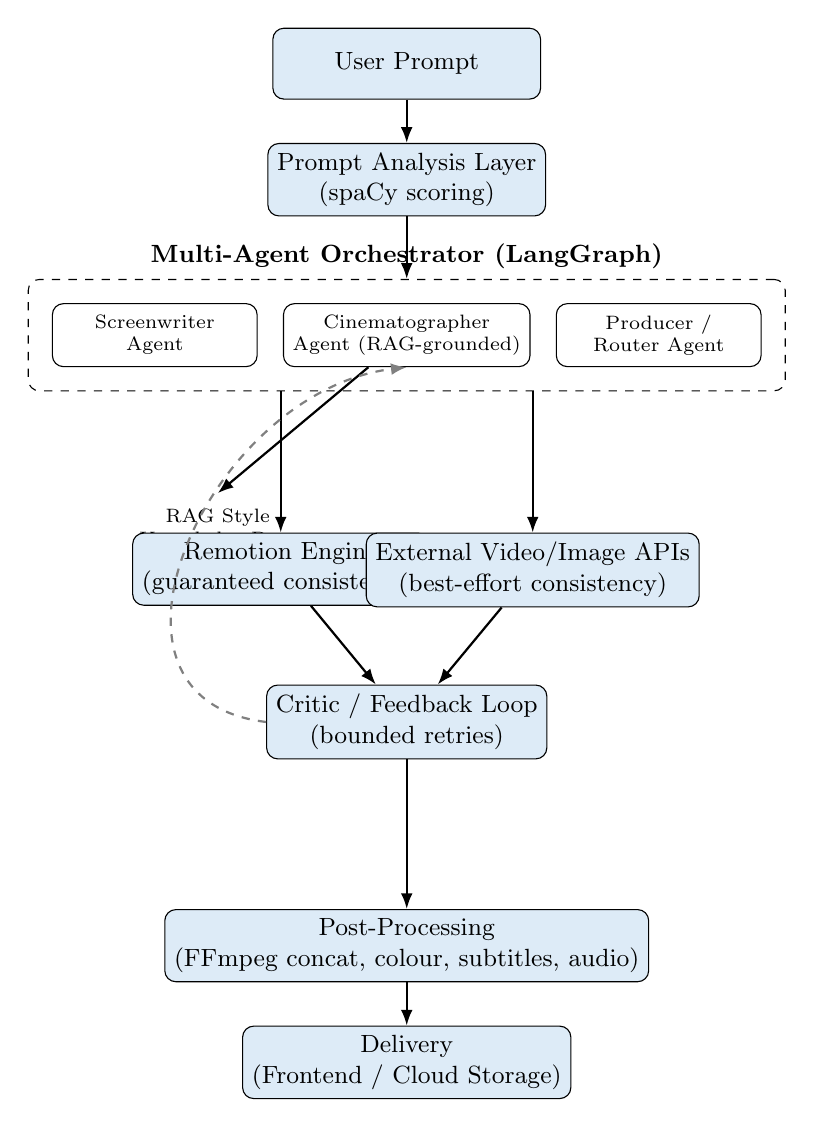
\begin{tikzpicture}[
    node distance=0.55cm and 1.3cm,
    box/.style={draw, rounded corners, minimum width=3.4cm, minimum height=0.9cm, align=center, font=\small, fill=lightblue},
    agentbox/.style={draw, rounded corners, minimum width=2.6cm, minimum height=0.8cm, align=center, font=\scriptsize, fill=white},
    groupbox/.style={draw, dashed, rounded corners, inner sep=0.3cm},
    arr/.style={-{Latex[length=2mm]}, thick},
    dashedarr/.style={-{Latex[length=2mm]}, thick, dashed, gray}
]

\node[box] (input) {User Prompt};
\node[box, below=of input] (analysis) {Prompt Analysis Layer\\(spaCy scoring)};

\node[agentbox, below=1.1cm of analysis, xshift=-3.2cm] (screenwriter) {Screenwriter\\Agent};
\node[agentbox, below=1.1cm of analysis] (cinematographer) {Cinematographer\\Agent (RAG-grounded)};
\node[agentbox, below=1.1cm of analysis, xshift=3.2cm] (producer) {Producer /\\Router Agent};

\node[groupbox, fit=(screenwriter)(cinematographer)(producer), label={[font=\small\bfseries]above:Multi-Agent Orchestrator (LangGraph)}] (orchestrator) {};

\node[box, draw=none, fill=none, below=1.6cm of cinematographer, xshift=-2.4cm, font=\scriptsize] (ragstore) {RAG Style\\Knowledge Base};

\node[box, below=2.1cm of screenwriter, xshift=1.6cm] (remotion) {Remotion Engine\\(guaranteed consistency)};
\node[box, below=2.1cm of producer, xshift=-1.6cm] (apis) {External Video/Image APIs\\(best-effort consistency)};

\node[box, below=1.0cm of remotion, xshift=1.6cm] (critic) {Critic / Feedback Loop\\(bounded retries)};

\node[box, below=1.9cm of critic] (postproc) {Post-Processing\\(FFmpeg concat, colour, subtitles, audio)};
\node[box, below=of postproc] (delivery) {Delivery\\(Frontend / Cloud Storage)};

\draw[arr] (input) -- (analysis);
\draw[arr] (analysis) -- (orchestrator.north);
\draw[arr] (cinematographer) -- (ragstore.north);
\draw[arr] (orchestrator.south -| remotion.north) -- (remotion.north);
\draw[arr] (orchestrator.south -| apis.north) -- (apis.north);
\draw[arr] (remotion) -- (critic);
\draw[arr] (apis) -- (critic);
\draw[dashedarr] (critic.west) .. controls +(-2.5,0.3) and +(-2.5,-0.3) .. (cinematographer.south);
\draw[arr] (critic) -- (postproc);
\draw[arr] (postproc) -- (delivery);

\end{tikzpicture}
\caption{VidCraft architecture: prompt analysis feeds a LangGraph multi-agent orchestrator; the Cinematographer agent grounds style decisions via retrieval; shots are routed to the Remotion or external-API pathway; a bounded critic loop (dashed arrow) may trigger limited re-generation before post-processing and delivery.}
\label{fig:architecture}
\end{figure}

\begin{figure}[htbp]
\centering
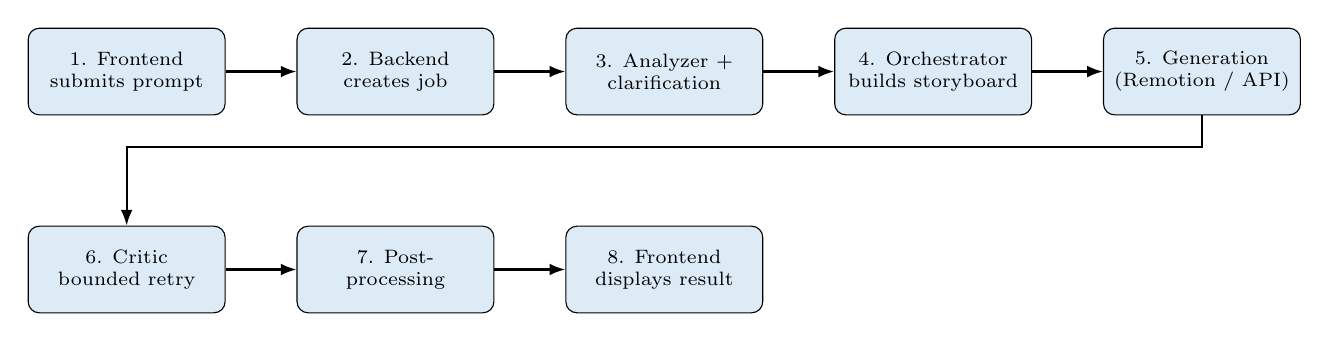
\begin{tikzpicture}[
    node distance=0.9cm,
    seqbox/.style={draw, rounded corners, minimum width=2.5cm, minimum height=1.1cm, align=center, font=\scriptsize, fill=lightblue},
    arr/.style={-{Latex[length=2mm]}, thick}
]
\node[seqbox] (s1) {1. Frontend\\submits prompt};
\node[seqbox, right=of s1] (s2) {2. Backend\\creates job};
\node[seqbox, right=of s2] (s3) {3. Analyzer +\\clarification};
\node[seqbox, right=of s3] (s4) {4. Orchestrator\\builds storyboard};
\node[seqbox, right=of s4] (s5) {5. Generation\\(Remotion / API)};

\node[seqbox, below=1.4cm of s3] (s8) {8. Frontend\\displays result};
\node[seqbox, left=of s8] (s7) {7. Post-\\processing};
\node[seqbox, left=of s7] (s6) {6. Critic\\bounded retry};

\draw[arr] (s1) -- (s2);
\draw[arr] (s2) -- (s3);
\draw[arr] (s3) -- (s4);
\draw[arr] (s4) -- (s5);
\draw[arr] (s5.south) -- ++(0,-0.4) -| (s6.north);
\draw[arr] (s6) -- (s7);
\draw[arr] (s7) -- (s8);
\end{tikzpicture}
\caption{End-to-end request sequence for a single generation, corresponding to the architecture in Figure~\ref{fig:architecture}.}
\label{fig:sequence}
\end{figure}

\needspace{0.5\textheight}
\section{Individual Tasks}

Task ownership follows a vertical-slice model: each member owns one architectural layer end-to-end (AI/orchestration, backend, frontend, or NLP/RAG research) rather than being assigned isolated, disconnected tickets, so that integration responsibility is clear throughout the timeline.

\begin{center}
\begin{longtable}{|p{2.2cm}|p{5.9cm}|p{3.4cm}|p{2.1cm}|}
\hline
\tblhead{Member} & \tblhead{Individual Tasks} & \tblhead{Key Deliverable} & \tblhead{Tentative Date} \\
\hline
\endfirsthead
\hline
\tblhead{Member} & \tblhead{Individual Tasks} & \tblhead{Key Deliverable} & \tblhead{Tentative Date} \\
\hline
\endhead

\multirow{7}{2.2cm}{Muhammad Majid (Lead)}
 & Technology feasibility testing; Python environment setup (spaCy, sentence-transformers, LangChain/LangGraph, Groq SDK, OpenCV, FFmpeg) & Verified working dev environment & May 2026 \\
 & FastAPI microservice scaffolding; spaCy prompt-analysis pipeline implementation & Prompt analyzer returning structured scores & Jun -- Jul 2026 \\
 & LangGraph multi-agent orchestrator: Screenwriter and Producer/Router agents; Groq and fallback LLM integration & Working storyboard decomposition & Aug -- Oct 2026 \\
 & Critic and quality-feedback loop implementation, including bounded retry logic and structured feedback parsing & Demonstrated retry cycle & Nov -- Dec 2026 \\
 & Backend--AI service communication optimisation and orchestrator refinement & Stable orchestrator under repeated runs & Jan 2027 \\
 & Evaluation study execution (baseline vs.\ multi-agent comparison) and results analysis & Evaluation results table & Feb 2027 \\
 & Architecture documentation; final demo narration and technical walkthrough & Final report chapter; demo script & Mar -- Apr 2027 \\
\hline

\multirow{7}{2.2cm}{Tahir Zaka}
 & Node.js and Express project setup, MongoDB configuration, Redis setup, GitHub repository management & Working backend scaffold & May 2026 \\
 & REST API routes, security middleware, logging, database schema design & Documented API contract & Jun 2026 \\
 & Job queue and WebSocket integration; Remotion render job orchestration & Async job pipeline with live status updates & Jul -- Aug 2026 \\
 & Vector index integration to support RAG retrieval backend & Queryable style-vector index & Sep -- Nov 2026 \\
 & External video/image API integration and tiered provider selection logic & Working tiered provider fallback & Nov -- Dec 2026 \\
 & FFmpeg backend integration, including multi-shot concatenation; cloud media hosting; file management & Concatenated multi-shot MP4 output & Jan 2027 \\
 & Backend optimisation, deployment testing, reports & Deployment-ready backend & Feb -- Apr 2027 \\
\hline

\multirow{5}{2.2cm}{Hammad}
 & React/Vite project setup with Tailwind CSS and UI component integration & Working frontend scaffold & May -- Jun 2026 \\
 & Prompt input interface and conversational clarification chat UI & Functional clarification chat flow & Jul 2026 \\
 & Style configurator and storyboard/shot timeline visualisation & Interactive storyboard view & Aug -- Sep 2026 \\
 & Real-time progress tracking interface, video display panel, prompt/version history & Live progress UI over WebSocket & Oct -- Nov 2026 \\
 & Responsive refinement, error handling, loading states, frontend documentation & Mobile-responsive, documented UI & Dec 2026 -- Apr 2027 \\
\hline

\multirow{6}{2.2cm}{Maida Ibrar}
 & NLP Python environment setup, Jupyter configuration, spaCy entity-recognition validation & Validated NLP dev environment & May -- Jun 2026 \\
 & Cinematography reference corpus curation (shot types, lighting, genre conventions) for the RAG knowledge base & Curated, cleaned reference corpus & Jul -- Aug 2026 \\
 & RAG retrieval module: embedding generation, vector index population, Cinematographer agent grounding logic & Working retrieval-grounded style step & Sep -- Oct 2026 \\
 & Continuity/world-state schema design; contradiction dictionary development & Documented world-state schema & Nov 2026 \\
 & End-to-end integration testing; evaluation dataset curation & Curated 50-prompt evaluation set & Dec 2026 -- Jan 2027 \\
 & Literature review, evaluation study support, report writing & Related Work chapter; evaluation write-up & Feb -- Apr 2027 \\
\hline
\end{longtable}
\end{center}

\needspace{0.5\textheight}
\section{Gantt Chart}

The project is organised into ten development phases spanning twelve months, from May 2026 to April 2027.

\begin{center}
\begin{tabular}{|p{4.1cm}|c|c|c|c|c|c|c|c|c|c|c|c|}
\hline
\rowcolor{headerblue}
\textcolor{white}{\textbf{Phase}} &
\rotatebox{90}{\textcolor{white}{May 26}} &
\rotatebox{90}{\textcolor{white}{Jun 26}} &
\rotatebox{90}{\textcolor{white}{Jul 26}} &
\rotatebox{90}{\textcolor{white}{Aug 26}} &
\rotatebox{90}{\textcolor{white}{Sep 26}} &
\rotatebox{90}{\textcolor{white}{Oct 26}} &
\rotatebox{90}{\textcolor{white}{Nov 26}} &
\rotatebox{90}{\textcolor{white}{Dec 26}} &
\rotatebox{90}{\textcolor{white}{Jan 27}} &
\rotatebox{90}{\textcolor{white}{Feb 27}} &
\rotatebox{90}{\textcolor{white}{Mar 27}} &
\rotatebox{90}{\textcolor{white}{Apr 27}} \\
\hline
1. Research \& Env.\ Setup & \cellcolor{gray!60} & & & & & & & & & & & \\
\hline
2. Backend, DB \& Vector Index & & \cellcolor{gray!60} & & & & & & & & & & \\
\hline
3. Frontend Development & & \cellcolor{gray!60} & \cellcolor{gray!60} & & & & & & & & & \\
\hline
4. Remotion Integration & & & \cellcolor{gray!60} & \cellcolor{gray!60} & & & & & & & & \\
\hline
5. Multi-Agent Orchestration \& NLP Core & & & & \cellcolor{gray!60} & \cellcolor{gray!60} & \cellcolor{gray!60} & & & & & & \\
\hline
6. RAG Knowledge Base \& Style Grounding & & & & & \cellcolor{gray!60} & \cellcolor{gray!60} & \cellcolor{gray!60} & & & & & \\
\hline
7. Critic Loop \& API Integration & & & & & & & \cellcolor{gray!60} & \cellcolor{gray!60} & & & & \\
\hline
8. Integration \& Optimization & & & & & & & & & \cellcolor{gray!60} & & & \\
\hline
9. Evaluation Study & & & & & & & & & & \cellcolor{gray!60} & & \\
\hline
10. Report Writing \& Demo Prep & & & & & & & & & & & \cellcolor{gray!60} & \cellcolor{gray!60} \\
\hline
\end{tabular}
\end{center}

\subsection*{Key Milestones}
\begin{itemize}[leftmargin=*]
\item \textbf{M1 (May 2026)} -- Development environment and technology feasibility confirmed.
\item \textbf{M2 (Jun 2026)} -- Backend scaffold, database and job queue operational.
\item \textbf{M3 (Jul 2026)} -- Frontend scaffold and prompt input interface operational.
\item \textbf{M4 (Aug 2026)} -- Remotion pathway renders a first end-to-end animated composition.
\item \textbf{M5 (Oct 2026)} -- Multi-agent orchestrator produces a coherent multi-shot storyboard.
\item \textbf{M6 (Nov 2026)} -- RAG-grounded style retrieval integrated into the Cinematographer agent.
\item \textbf{M7 (Dec 2026)} -- Critic-and-retry loop and external API pathway operational.
\item \textbf{M8 (Jan 2027)} -- Full system integration complete; end-to-end run succeeds.
\item \textbf{M9 (Feb 2027)} -- Evaluation study completed and results documented.
\item \textbf{M10 (Apr 2027)} -- Final report submitted; live demonstration delivered.
\end{itemize}

\needspace{0.5\textheight}
\section{Tools and Technologies}

\subsection{Agent Orchestration and Retrieval}
\begin{itemize}[leftmargin=*]
\item \textbf{LangChain and LangGraph} for multi-agent orchestration and state management -- chosen over a hand-rolled if/else pipeline because the state-graph model gives explicit, inspectable control flow, conditional branching and bounded cycles for the retry logic.
\item \textbf{Groq API} for low-latency, primary LLM inference within the agent graph -- chosen because the orchestrator issues multiple sequential calls per generation, where inference latency compounds noticeably.
\item \textbf{Fallback LLM API} (e.g.\ OpenAI GPT) for higher-complexity reasoning and vision-based critic scoring, used selectively rather than as the default path.
\item \textbf{sentence-transformers} (\texttt{all-MiniLM-L6-v2}) for embeddings, used for both prompt-intent similarity checks and RAG retrieval.
\item \textbf{Vector similarity search} (a FAISS index synced with MongoDB metadata) for RAG retrieval -- chosen for simplicity and to avoid depending on a separate managed vector-database service.
\end{itemize}

\subsection{Programmatic Video Generation -- Remotion}
\begin{itemize}[leftmargin=*]
\item Remotion for programmatic video generation
\item React components for animated video compositions
\item FFmpeg integration for MP4 rendering
\item CSS timeline animations using \texttt{useCurrentFrame}, \texttt{spring} and \texttt{interpolate}
\item Manim as an optional alternative for mathematical/educational visualisations
\end{itemize}

\subsection{Video and Image Generation API Strategy}
\textbf{Tier 1 -- Free-tier providers:} prioritised first for all development and testing.\\
\textbf{Tier 2 -- Affordable paid providers:} used when free-tier quotas are exhausted.\\
\textbf{Tier 3 -- Premium providers:} reserved for final demonstration and evaluation runs where higher fidelity is needed.

\subsection{Language Model APIs for Prompt Enhancement}
\begin{itemize}[leftmargin=*]
\item Groq-hosted open-weight models -- primary inference engine for the agent orchestration layer
\item A fallback cloud LLM API, selected based on cost and availability, for steps requiring stronger reasoning or multimodal (vision) capability
\end{itemize}

\subsection{Audio Generation (Optional)}
\begin{itemize}[leftmargin=*]
\item A single free-tier text-to-speech provider for narration synthesis
\item FFmpeg audio stream merging and synchronisation
\end{itemize}

\subsection{Frontend, Backend and DevOps Stack}

\begin{center}
\begin{tabular}{|l|l|l|l|}
\hline
\tblhead{Frontend} & \tblhead{Backend} & \tblhead{AI Microservice} & \tblhead{DevOps / Testing} \\
\hline
React & Node.js & Python & Git and GitHub \\
Vite & Express.js & FastAPI & Postman \\
Tailwind CSS & MongoDB + Mongoose & Uvicorn & Python unittest / pytest \\
shadcn/ui & Job queue (Bull.js) & spaCy & Jupyter Notebook \\
Zustand & Redis & LangChain / LangGraph & \\
Recharts & Socket.IO Server & sentence-transformers & \\
Framer Motion & Morgan, Helmet & scikit-learn, NumPy & \\
Socket.IO Client & Cloud media hosting & OpenCV, Pillow & \\
Axios, React Query & & FFmpeg & \\
\hline
\end{tabular}
\end{center}

\needspace{0.5\textheight}
\section{References}

\begin{thebibliography}{99}

\bibitem{sora} OpenAI. (2024). \textit{Sora: Video Generation Models as World Simulators}. OpenAI Technical Report.

\bibitem{veo} Google DeepMind. (2024). \textit{Veo: A Large-Scale Video Generation Model}. Google Technical Report.

\bibitem{controllable_survey} Ma, Y., et al. (2026). \textit{Controllable Video Generation: A Survey}. arXiv preprint arXiv:2507.16869.

\bibitem{devil_in_prompts} Liu, Y., et al. (2025). \textit{The Devil is in the Prompts: Retrieval-Augmented Prompt Optimization for Text-to-Video Generation}. CVPR 2025.

\bibitem{phyt2v} PhyT2V Research Team. (2025). \textit{PhyT2V: LLM-Guided Iterative Self-Refinement for Physics-Grounded Text-to-Video Generation}. CVPR 2025.

\bibitem{selfrefine} Madaan, A., et al. (2023). \textit{Self-Refine: Iterative Refinement with Self-Feedback}. NeurIPS 2023.

\bibitem{genagents} Park, J. S., et al. (2023). \textit{Generative Agents: Interactive Simulacra of Human Behavior}. UIST 2023.

\bibitem{langgraph} LangChain. (2024). \textit{LangGraph: Building Stateful, Multi-Agent Applications with LLMs}. \url{https://www.langchain.com/langgraph}

\bibitem{rag} Lewis, P., et al. (2020). \textit{Retrieval-Augmented Generation for Knowledge-Intensive NLP Tasks}. NeurIPS 2020.

\bibitem{clipscore} Hessel, J., et al. (2021). \textit{CLIPScore: A Reference-free Evaluation Metric for Image Captioning}. EMNLP 2021.

\bibitem{stable_cinemetrics} Stable Cinemetrics Team. (2025). \textit{Stable Cinemetrics: Structured Taxonomy and Evaluation for Professional Video Generation}. NeurIPS 2025.

\bibitem{remotion} Burger, J. (2021). \textit{Remotion: Create Videos Programmatically in React}. \url{https://www.remotion.dev}

\bibitem{sbert} Reimers, N., \& Gurevych, I. (2019). \textit{Sentence-BERT: Sentence Embeddings using Siamese BERT-Networks}. Proceedings of EMNLP 2019.

\bibitem{spacy} Honnibal, M., \& Montani, I. (2017). \textit{spaCy 2: Natural Language Understanding with Bloom Embeddings, Convolutional Neural Networks and Incremental Parsing}.

\bibitem{evalcrafter} EvalCrafter Team. (2024). \textit{EvalCrafter: Benchmarking and Evaluating Large Video Generation Models}. CVPR 2024.

\bibitem{manim} Manim Community. (2021). \textit{Manim -- Mathematical Animation Engine}. \url{https://www.manim.community}

\end{thebibliography}

\appendix

\section{Example Prompt Analysis Output}
See Section~6.1 for the full example. The analyzer's JSON schema is stable across the project and used as the contract between the FastAPI microservice and the Node.js backend.

\section{Example Storyboard Object}
See Section~6.3 for the full example. The \texttt{world\_state} object shown there is the same object propagated through generation as described in Section~6.6.

\section{Example Critic Feedback Object}

\begin{verbatim}
{
  "shot_id": 2,
  "passed": false,
  "reason": "Background lighting does not match 'warm dusk
             lighting' style token; appears daytime-lit.",
  "suggested_revision": "Increase warm colour temperature and
                          add long shadow cues to the prompt."
}
\end{verbatim}

\end{document}
